
\documentclass[a4paper]{article}

%% Language and font encodings
\usepackage[english]{babel}
\usepackage[T1]{fontenc}

%% Sets page size and margins
\usepackage[a4paper,top=3cm,bottom=2cm,left=3cm,right=3cm,marginparwidth=1.75cm]{geometry}

%% Useful packages
\usepackage{amsmath}
\usepackage{graphicx}
\usepackage{float}
\usepackage[colorinlistoftodos]{todonotes}
\usepackage[colorlinks=true, allcolors=blue]{hyperref}

\title{Animal Morphing using Deep Convolutional Generative Adversarial Networks}
\author{
	You
}

\begin{document}
\maketitle

%\begin{abstract}
%Your abstract.
%\end{abstract}

\section{Introduction}
In this project, we will implement Deep Convolutional Generative Adversarial Networks (DCGANs)  \cite{DBLP:journals/corr/RadfordMC15} for image processing. We will use a subset of CIFAR-100 dataset containing only animals. Our aim will be three-fold; we will first implement a photo-realistic animal generator, then allow users to sketch animals and have this sketch morphed into a photo-realistic animal, then finally allow users to restrict the class of the generated animal. The first part is of high-priority, the second and third ones could be optional since they are partially out of the scope of deep learning.


%
%
%
\section{Random Generator}
We will start by implementing the model as in \cite{DBLP:journals/corr/RadfordMC15}. The model is thoroughly described in the paper and there are sufficient available resources.

\begin{figure}[H]
	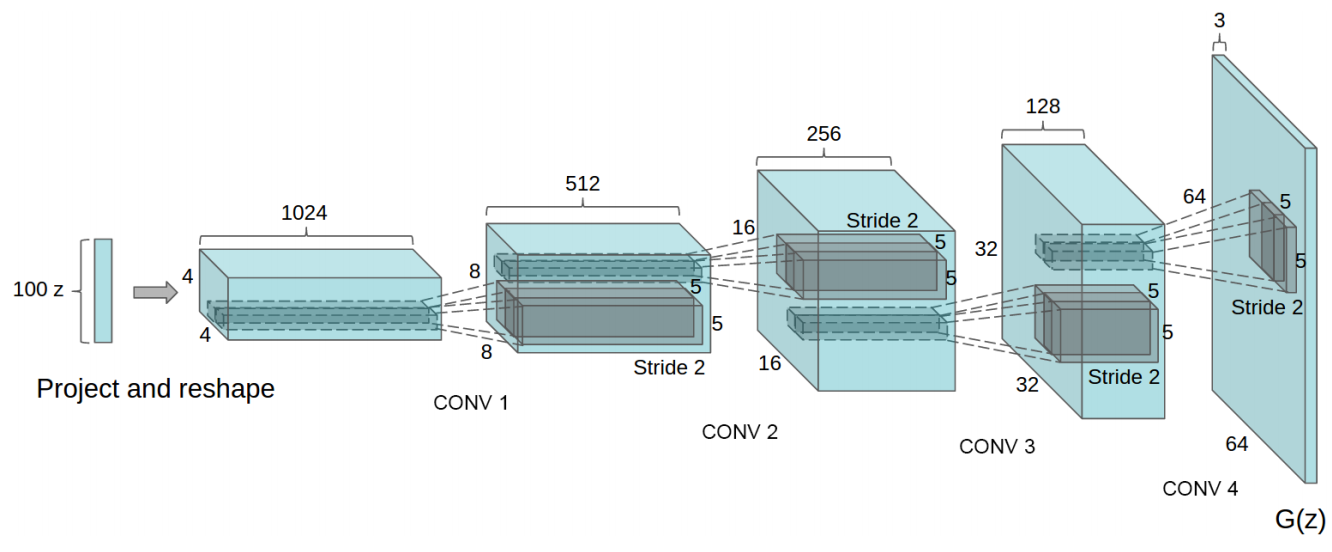
\includegraphics[width=\textwidth]{DCGAN.png}
	\caption{Generator network. Picture from \cite{DBLP:journals/corr/RadfordMC15}. }
\end{figure}

We will start by using CIFAR-100 and take a subset of 60 classes including [...]. The images in this dataset are 32 $\times$ 32 $\times$ 3.



%
%
%
\section{Sketch-to-Picture Generator}

On top of the previous part, we will implement a simple UI to allow users to sketch and have photo-realistic images of animals generated from their sketch. Here, we will use the discriminator network to infer the latent representation of the sketch and then feed this into the generator to create the image.

We have experience building web-based UIs in the project team, so to minimize implementation time we will certainly use it and implement a simple React web-app and an API endpoint for our trained model.  

%
%
%
\section{Constrained Sketch-to-Picture Generator}
On top of the previous part, we will add a field to allow users to restrict the class of the generated animal. That is, if the user's drawing ressembles a cat but this restriction field is set to "


\bibliographystyle{alpha}
\bibliography{bib}
\end{document}